Like any program analysis tool, a mechanism is required to collect data about the program behavior.

\begin{itemize}
\item \hl{Static vs. Dynamic}
\item \hl{Sampling and hardware counters like TAU and Score-p vs Whole program analysis}
\item \hl{pros and cons of each, a small fraction of related work on tracing}
\end{itemize}

We have used ParLOT \cite{parlot} to collect our data.
%
ParLOT is an efficient tracing tool that captures all function calls and returns at different levels via dynamic binary instrumentation \cite{pin}.
%
ParLOT incrementally compresses the captured function calls and returns on-the-fly, resulting in highly compressed trace files that occupy only a few kilobytes on the disk and leave the majority of bandwidth for the network and system.
%
Upon termination of the application execution, either a ``successful’’ termination or ``failure’’ of the application due to crash, deadlock (T/O) or corrupted result, a Compressed ParLOT Trace (CPT) for each executing thread would be generated. Each $CPT_i$ then be \textit{pre-processed} (e.g., decompressed, filtered, etc. more in section \ref{subsec:nlr}) and form  $PT_i$ where $i$ is the index of process/thread.
%
Our strategy is to perform a post mortem analysis on PTs to study different aspects of application dynamic behavior.
%
Our main focus is the comparison between a successful run and failed run.
%
Such an approach has proven to be useful in works such as delta debugging \cite{choi-concurentDelta} where an application used to work fine yesterday but failed today due to various factors such as a change in the source code, an API library update, use of a different compiler or porting to a new system.

\subsection{Odd/Even Sort Example}

For a better explanation of our idea, we explain our approaches on a simple parallel (MPI) implementation of odd/even sort \hl{[cite the git url]}.

Odd/Even sort is a variant of the bubble-sort operates in two alternate phases: \textit{Phase-even} where even processes exchange (compare and swap) values with right neighbors and \textit{Phase-odd} where odd processes exchange values with right neighbors. Figure \ref{fig.oddEven} shows the simplified MPI implementation of the odd/even sort algorithm.


The for loop in line 4 of \texttt{oddEvenSort()} iterates over phases of the algorithm and based on the phase, the appropriate partner for each rank is getting discovered by the function \texttt{findPtr()} (line 6). The odd/even ranks then exchange their chunks of data (lines 9-13) and a set of sort, merge and copy operations would be performed on received data by each rank (which are replaced by \texttt{...} in line 15 for simplicity).

\begin{figure}[]
\centering
\caption{Simplified MPI implementation of Odd/Even Sort}
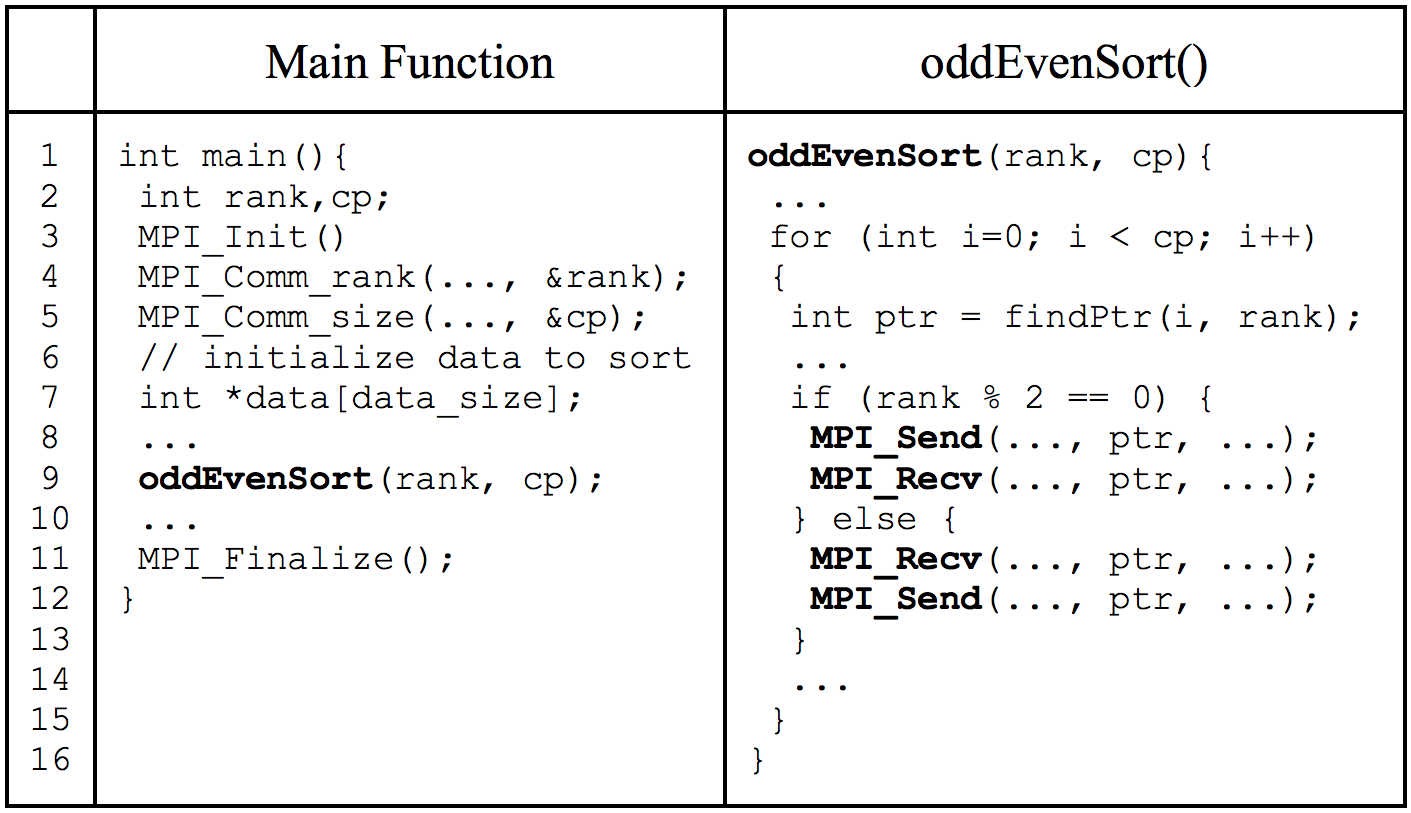
\includegraphics[width=0.45\textwidth]{figs/oddEven.png}
\label{fig.oddEven}
\end{figure}


Execution of odd/even sort application with four processes (\texttt{mpirun -np 4}) while ParLOT trace collection is enabled on top of the application, would result in 4 PTs (table \ref{tab:oddEvenPT}). This execution terminates successfully with expected results and the set of generated PTs clearly reflects the expected behavior (control flow) of odd and even processes.
%
\\
Now let's swap the the order of MPI\_Recv and MPI\_Send in lines 11 and 12 (figure \ref{fig.oddEvenDL}). According to MPI Standard  \hl{[cite MPI-forum or openMPI url]}, MPI\_Send is a \textit{blocking send} used the \textit{standard} communication mode. In this mode,  MPI may buffer outgoing messages and the send call may complete before a matching receive is invoked. On the other hand, buffer space may be unavailable, or MPI may choose not to buffer outgoing messages, for performance reasons. In this case, the send call will not complete until a matching receive has been posted, and the data has been moved to the receiver. This shows that, based on the MPI implementation, the \texttt{oddEvenSort\_DL()} might end up causing a deadlock.


\begin{table}[]
\centering
\caption{The generated PTs for odd/even execution with four processes}
\label{tab:oddEvenPT}
\scalebox{0.75}{
\begin{tabular}{|l|l|l|l|}
\hline
\rowcolor[HTML]{EFEFEF} 
\multicolumn{1}{|c|}{\cellcolor[HTML]{EFEFEF}\textbf{$PT_0$}} & \multicolumn{1}{c|}{\cellcolor[HTML]{EFEFEF}\textbf{$PT_1$}} & \multicolumn{1}{c|}{\cellcolor[HTML]{EFEFEF}\textbf{$PT_2$}} & \multicolumn{1}{c|}{\cellcolor[HTML]{EFEFEF}\textbf{$PT_3$}} \\ \hline \hline
... & ... & ... & ... \\ \\[-1em]  \hline
main & main & main & main \\ \\[-1em]  \hline
MPI\_Init & MPI\_Init & MPI\_Init & MPI\_Init \\ \\[-1em]  \hline
MPI\_Comm\_Rank & MPI\_Comm\_Rank & MPI\_Comm\_Rank & MPI\_Comm\_Rank \\ \\[-1em]  \hline
MPI\_Comm\_Size & MPI\_Comm\_Size & MPI\_Comm\_Size & MPI\_Comm\_Size \\ \\[-1em]  \hline
... & ... & ... & ... \\ \\[-1em]  \hline
oddEvenSort & oddEvenSort & oddEvenSort & oddEvenSort \\ \\[-1em]  \hline
... & ... & ... & ... \\ \\[-1em] \hline
findPtr & findPtr & findPtr & findPtr \\ \hline
\rowcolor[HTML]{FFCCC9} 
{\color[HTML]{333333} MPI\_Send} & \cellcolor[HTML]{CBCEFB}{\color[HTML]{333333} MPI\_Recv} & {\color[HTML]{333333} MPI\_Send} & \cellcolor[HTML]{CBCEFB}{\color[HTML]{333333} MPI\_Recv} \\ \hline
\rowcolor[HTML]{FFCCC9} 
{\color[HTML]{333333} MPI\_Recv} & \cellcolor[HTML]{CBCEFB}{\color[HTML]{333333} MPI\_Send} & {\color[HTML]{333333} MPI\_Recv} & \cellcolor[HTML]{CBCEFB}{\color[HTML]{333333} MPI\_Send} \\ \hline
... & ... & ... & ... \\ \hline
findPtr & findPtr & findPtr & findPtr \\ \hline
\rowcolor[HTML]{FFCCC9} 
{\color[HTML]{333333} MPI\_Send} & \cellcolor[HTML]{CBCEFB}{\color[HTML]{333333} MPI\_Recv} & {\color[HTML]{333333} MPI\_Send} & \cellcolor[HTML]{CBCEFB}{\color[HTML]{333333} MPI\_Recv} \\ \hline
\rowcolor[HTML]{FFCCC9} 
{\color[HTML]{333333} MPI\_Recv} & \cellcolor[HTML]{CBCEFB}{\color[HTML]{333333} MPI\_Send} & {\color[HTML]{333333} MPI\_Recv} & \cellcolor[HTML]{CBCEFB}{\color[HTML]{333333} MPI\_Send} \\ \hline
... & ... & ... & ... \\ \hline
MPI\_Finalize & MPI\_Finalize & MPI\_Finalize & MPI\_Finalize \\ \hline
\end{tabular}}
\end{table}


\begin{figure}[]
\centering
\caption{A line change in oddEvenSort (left) that might cause a deadlock in oddEvenSort\_DL (right)}
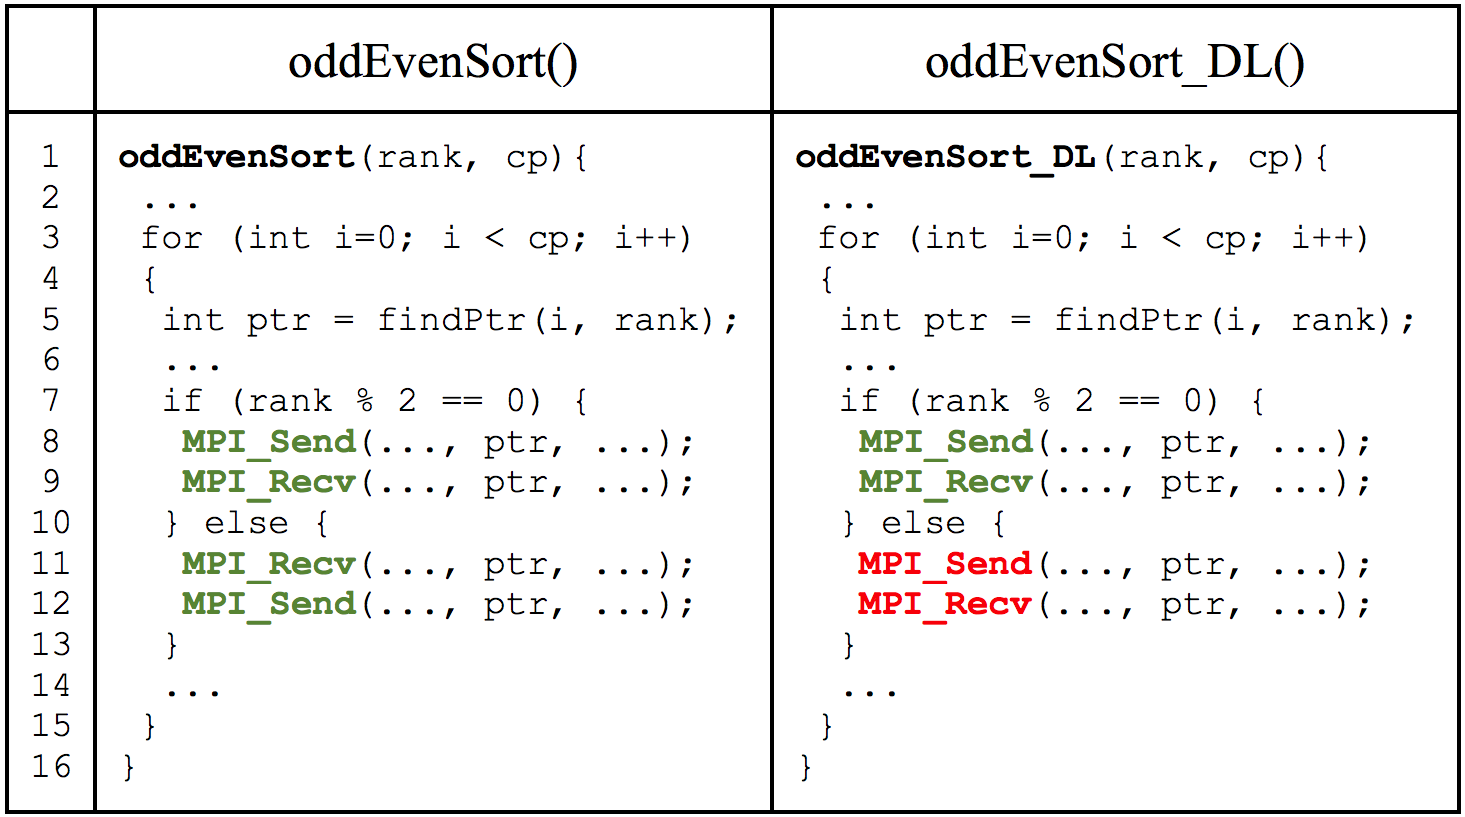
\includegraphics[width=0.45\textwidth]{figs/oddEvenDL.png}
\label{fig.oddEvenDL}
\end{figure}


HPC applications often execute on supercomputers with multiple levels of parallelism from distributed systems (MPI) to shared memory (OpenMP) and accelerators (GPU). Finding flaws like the one in figure \ref{fig.oddEvenDL} in such an environment is the problem of \textit{finding the needle in the haystack}.
%
\begin{itemize}
\item Trade-off between collecting sufficient information and adding reasonable overhead to the native execution is solved with ParLOT
\item However, generated PTs by ParLOT are difficult to analyze (thousands of long sequences of function calls and returns)
\item Solution:
	\begin{itemize}
	\item intra-PT compression (decompress, filter and NLR: section \ref{subsec:nlr})
	\item inter-PT compression (Concept Lattices: section \ref{subsec:fca})
	\item Locating suspicious PTs that might suffer from a flaw: section \ref{subsec:ranking} and delta comparison (diffNLR section: \ref{subsec:diffnlr})
	\end{itemize}
\end{itemize}


\clearpage

% NLRs
\subsection{Pre-Processing CPTs}
\label{subsec:nlr}

\begin{itemize}
	\item Decompress and Filters
	\begin{itemize}
		\item ParLOT leaves Compressed Traces (CPTs)
		\item CPTs need to be decompressed and decoded to PTs 
		\item Each PT contains a full sequence of ordered function calls. Not all of the functions are in our interest - Hierarchy of filters: Table \ref{tab:filters}.  
	\end{itemize}
	\item Loops in source codes would be reflected in PTs as sequences of repetitive patterns.
	\item HPC applications and resources are of great interest to scientists and engineers for simulating \textit{iterative} kernels. Computer simulation of fluid dynamics, partial differential equations, the Gauss-Seidel method, and finite element methods in form of stencil codes, all include a main outer loop that iterates over some elements (i.e., timesteps) and updates the elements.
	\item Mining loops advantages:
	\begin{itemize}
		\item Lossless compression (intra-PT), making long PTs easier to analyze and read
		\item broken loop structures due to a fault would be revealed
		\item Others have done the same (STAT, AutomaDeD, PRODOMETER) 
	\end{itemize}
	\item We have adopted ideas from Kobayashi \cite{kobayashi-84} (definition of loops) and \cite{Ketterlin-nlr} (NLR algorithm)
	\item We have slightly changed the NLR algorithm to make it suitable for PT contents.
	 
	\item explanations on loop structures, loop bodies and loop counts, example \ref{fig.NLRexample}
	\item NLR algorithm and complexity
\end{itemize}

% Please add the following required packages to your document preamble:
% \usepackage{multirow}
\begin{table}[]
\centering
\caption{Applicable filters to PT contents based on regular expressions}
\label{tab:filters}
\scalebox{0.65}{
\begin{tabular}{|c|c|l|}
\hline
\textbf{Category} & \textbf{Sub-Category} & \multicolumn{1}{c|}{\textbf{Description}} \\ \hline
\multirow{2}{*}{Primary} & Returns & Filter out all returns \\ \cline{2-3} 
 & PLT & \begin{tabular}[c]{@{}l@{}}Filter out the ".plt" function calls for external functions/procedures that \\ their address needs to be resolved dynamically from Procedure Linkage \\ Table (PLT)\end{tabular} \\ \hline
\multirow{4}{*}{MPI} & MPI All & Only keep functions that start with "MPI\_" \\ \cline{2-3} 
 & MPI Collectives & Only keep MPI collective calls (MPI\_Barrier, MPI\_Allreduce, etc) \\ \cline{2-3} 
 & MPI Send/Recv & Only keep MPI\_Send, MPI\_Isend, MPI\_Recv, MPI\_Irecv and MPI\_Wait \\ \cline{2-3} 
 & MPI Internal Library & Keep all inner MPI library calls \\ \hline
\multirow{3}{*}{OMP} & OMP All & Only keep OMP calls (starting with GOMP\_) \\ \cline{2-3} 
 & OMP Critical & Only keep OMP\_CRITICAL\_START and OMP\_CRITICAL\_END \\ \cline{2-3} 
 & OMP Mutex & Only keep OMP\_Mutex calls \\ \hline
\multirow{4}{*}{System} & Memory & Keep any memory related functions (memcpy, memchk, alloc, malloc, etc) \\ \cline{2-3} 
 & Network & Keep any network related functions (network, tcp, sched, etc) \\ \cline{2-3} 
 & Poll & Keep any poll related functions (poll, yield, sched, etc) \\ \cline{2-3} 
 & String & Keep any string related functions (strlen, strcpy, etc) \\ \hline
\multirow{2}{*}{Advanced} & Custom & Any regular expression can be captured \\ \cline{2-3} 
 & Everything & Does not filter anything \\ \hline
\end{tabular}}
\end{table}


\begin{figure}[]
\caption{Sample NLR}
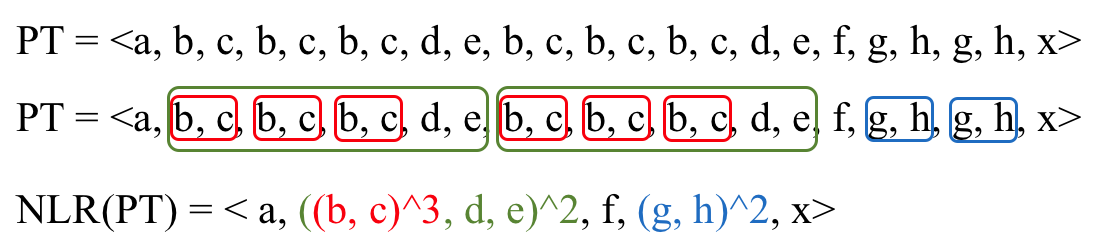
\includegraphics[width=0.45\textwidth]{figs/NLRexample.png}
\label{fig.NLRexample}
\end{figure}

\clearpage

\subsection{Equivalencing behavior via FCA}
\label{subsec:fca}

Thanks to ParLoT compression mechanism, we are able to efficiently (w.r.t. time and space) collect whole-program function call and return traces (PTs). However, post-mortem analysis of the PTs from thousands of threads requires decompression of traces, and consequently, analysis of large amount of data. Before jumping into \textit{the huge haystack} of PTs to find \textit{the tiny needle} (bug, bug manifestation or root cause of the failure), a middle ground data manipulation is required to simplify and organize the haystack. 

Reducing the search space from thousands of PTs to just a few groups of equivalent PTs (i.e., inter-PT compression) not only requires a similarity measure based on a call matrix but also a scheme that is efficient even for large process counts.
%
Since a pair-wise comparison of all processes is highly inefficient, we use \textit{concept lattices} that stem from \textit{formal concept analysis} (FCA) \cite{clbook} to store and compute groups of similar PTs.
%
FCA can efficiently split the large haystack into a few hay(semi)stacks with ``conceptually'' similar hays in each. This way conceptually isolated PTs (i.e., outliers) which are the potential bug manifestation or root cause would be detected. If no outlier detected, we only have a few distinct group of PTs to dig in, instead of thousands of large traces. With a wider perspective, here are other benefits of FCA for HPC debugging:
\begin{itemize}
\item FCA is scalable and efficient. It can be built incrementally and different kind of information such as full Jaccard Similarity Matrix (JSM) can be generated in linear time due to CL properties.
\item Clustering is only one advantage of creating concept lattices from ParLoT traces. CLs can integrate all traces from an execution to a single entity as signature/model of good or bad execution for further analysis (e.g., prediction) 
\item Due to the \textit{partial order} of nodes within CLs, valuable information can be retrieved from CLs like Happens-Before relation (Vijay Garg’s book explains all applications of FCA in computer science applications)\cite{latticeForDistConst} and machine learning and data mining \cite{Ignatov17})
\end{itemize}

A concept lattice is based on a \textit{formal context} \cite{clbook}, which is a triple $(O, A, I)$, where $O$ is a set of \textbf{objects}, $A$ a set of \textbf{attributes}, and $I \subseteq O \times A$ an incidence relation. The incidence relation associates each object with a set of attributes (e.g., table \ref{tab:sampleContext}).
%
Using FCA for clustering giving us the capability of clustering trace objects based on the ``concept'' of each trace object. We can characterize the ``concept'' (i.e., what we want to understand from the collected traces) by extracting meaningful ``attributes'' from traces. 
%
However, since we are only interested in grouping similar PTs in this work, we only take advantage of similarity measures \cite{Alqadah2011} of concept lattices and leave other properties for future work.
%
Due to typical HPC application topologies such as SPMD, master/worker and odd/even where multiple processes/threads behave similarly, our experiments show that large numbers of PTs can be reduced to just a few groups.
%

\subsubsection{Concept Lattice Construction}
\begin{itemize}
\item Batch vs. Incremental \cite{clconst}
\item Complexity: $O(2^{2K}||E||)$ where $K$ is an upper bound for number of attributes (e.g., distinct function calls in the whole execution) and $||E||$ is the number of objects (e.g., number of PTs).
\end{itemize}

\subsubsection{FCA example}

\begin{itemize}
	\item Construct the context table from example in figure \ref{fig.oddEven}
	\item Construct the Actual Concept Lattice from example in figure \ref{fig.oddEven}
\end{itemize}



\begin{table}[]
\label{tab:sampleContext}
\caption{Context}
\scalebox{0.6}{
\begin{tabular}{l|cccccc}
 & \multicolumn{1}{l}{MPI\_Init()} & \multicolumn{1}{l}{MPI\_Comm\_Size()} & \multicolumn{1}{l}{MPI\_Comm\_Rank()} & \multicolumn{1}{l}{MPI\_Send()} & \multicolumn{1}{l}{MPI\_Recv()} & \multicolumn{1}{l}{MPI\_Finalize()} \\ \hline
Rank 0 & $\times$ & $\times$ & $\times$ &  & $\times$ & $\times$ \\
Rank 1 & $\times$ & $\times$ & $\times$ & $\times$ &  & $\times$ \\
Rank 2 & $\times$ & $\times$ & $\times$ & $\times$ &  & $\times$ \\
Rank 3 & $\times$ & $\times$ & $\times$ & $\times$ &  & $\times$
\end{tabular}}
\end{table}


\begin{figure}[t]
\centering
\scalebox{0.5}{
\includegraphics[width=3.4in]{figs/{sample}.pdf}}
\caption{Sample Concept Lattice from Obj-Atr Context in table\ref{tab:sampleContext}}
\label{fig:sampleCL}
\end{figure}

\begin{figure}[t]
\centering
\scalebox{0.5}{
\includegraphics[width=3.4in]{figs/{sample-reduced}.pdf}}
\caption{Concept Lattice with reduced labels}
\label{fig:sampleCL}
\end{figure}





\subsubsection{Jaccard Similarity Scores}

\begin{itemize}
\item Some background about Jaccard Similarity Score
\item How to obtain full pair-wise Jaccard Similarity Matrix (JSM) from a concept lattice (e.g., LCA approach)
\end{itemize}

\begin{figure}[]
\centering
\scalebox{0.8}{
\includegraphics[width=3.4in]{figs/{fancy1}.pdf}}
\caption{Pair-wise Jaccard Similarity Matrix (JSM) of MPI processes in Sample code}
\label{fig:jsm}
\end{figure}


%\subsection{Ranking Suspicious PTs}
%\label{subsec:ranking}
%\begin{itemize}
%\item Filters
%\item Attributes
%\item 
%\end{itemize}



\subsection{diffNLR: Reflecting differences}
\label{subsec:diffnlr}
\begin{itemize}
\item Inspired by \texttt{diff} original algorithm\cite{diff-myers} that has bin used in Git and GNU Diff, we visualize the differences of a pair of PT as shown in fig \ref{fig:sampleDiffNLR}.
\item This visualization reflects of the differences of \textbf{occurrences} of PT elements and their \textbf{orders}.
\item In section \ref{sec:experimental} we show how this visualization can help us locating the points of divergence in PTs, and potential bug manifestation and root cause.
\end{itemize}

\begin{figure}[]
\centering
\scalebox{0.5}{
\includegraphics[width=3.4in]{figs/{sampleDiffNLR}.png}}
\caption{Sample diffNLR}
\label{fig:sampleDiffNLR}
\end{figure}


